\section{Datasets}
To show and explain the experiments, we need to look at some datasets we can evaluate our results. 
In this thesis, we primarily use four \todo{5} datasets to train and evaluate our results.

\subsection{kvasir}


Automatic computerised detection of diseases has been a quintessential focus on the medical industry, but for a long time, a still fairly unexplored research area.  As a response to this Simula Research laboratory together with \todo{more}, made the dataset Kvasir.
It was originally made to improve medical practice and refine health care systems where similar dataset did not exist.

Kvasir is a dataset containing images from inside the gastrointestinal tract containing three anatomical landmarks, in the form of (A), (B) and (C). Also, the Kvasir dataset includes two categories of images related to endoscopic polyp removal, (D) and (E). And lastly, three classes, (G), (H), and (I), containing images without the anomalies, as a form of baseline. 
Medical professionals sorted the dataset, and it is made to be used for both single and multi-disease computer-aided detection. 

At this time, there are two versions of the Kvasir dataset.  V1 vs V2
The images are from both from the lower and upper GI tract. 


\subsection{Nerthus} 
\todo{do we do Nerthus?}
\subsection{CVC-356}
\subsection{CVC-12k}
\subsection{CVC-612}


    
    
    %\textbf{The human digestive system may be affected by several diseases. Altogether esophageal, stomach and colorectal cancer accounts for about 2.8 million new cases and 1.8 million deaths per year. Endoscopic examinations are the gold standards for investigation of the GI tract. Gastroscopy is an examination of the upper GI tract including esophagus, stomach and first part of small bowel, while colonoscopy covers the large bowel (colon) and rectum. Both these examinations are real-time video examinations of the inside of the GI tract by use of digital high definition endoscopes. Endoscopic examinations are resource demanding and requires both expensive technical equipment and trained personnel. For colorectal cancer prevention, endoscopic detection and removal of possible precancerous lesions are essential. Adenoma detection is therefore considered to be an important quality indicator in colorectal cancer screening. However, the ability to detect adenomas varies between doctors, and this may eventually affect the individuals’ risk of getting colorectal cancer. Endoscopic assessment of severity and sub-classification of different findings may also vary from one doctor to another. Accurate grading of diseases are important since it may influence decision-making on treatment and follow-up. For example, the degree of inflammation directly affects the choice of therapy in inflammatory bowel diseases (IBD). An objective and automated scoring system would therefore be highly welcomed. Automatic detection, recognition and assessment of pathological findings will probably contribute to reduce inequalities, improve quality and optimize use of scarce medical resources. Furthermore, since endoscopic examinations are real-time investigations, both normal and abnormal findings have to be recorded and documented within written reports. Automatic report generation would proba- bly contribute to reduce doctors’ time required for paperwork and thereby increase time to patient care. Reliable and careful docu- mentation with the use of minimal standard terminology (MST) may also contribute to improved patient follow-up and treatment. To our knowledge, a standardized and automatic reporting system that ensure high quality endoscopy reports does not exist. In order to make the health care system more scalable and cost effective, basic research in the intersection between computer science and medicine must go beyond traditional medical imaging by combining this area with multimedia data analysis and retrieval, artificial intelligence, and distributed processing. Next-generation medical big-data applications are a frontier for innovation, compe- tition and productivity, where there are currently large initiatives both in the EU and the US. In the area of multimedia research, people are starting to see the synergies between multimedia and medical systems. For automatic algorithmic detection of abnormalities in the GI tract, there have been many proposals from various research communities, especially for the topic of polyp detection. However, the results are hard to reproduce due to lack of available medical data, i.e., the work listed above all use different and non-public data sets. Here, we therefore publish Kvasir: A Multi-Class Image Dataset for Computer Aided Gastrointestinal Disease Detection from the Vestre Viken Health Trust (Norway) containing not only polyps, but also two other findings, two classes related to polyp removal and three anatomical landmarks in the GI tract.}
    
\newpage
    
    %============================================
\iffalse
    \begin{figure}[t]
       \centering
        \subfloat[\centering g]{
            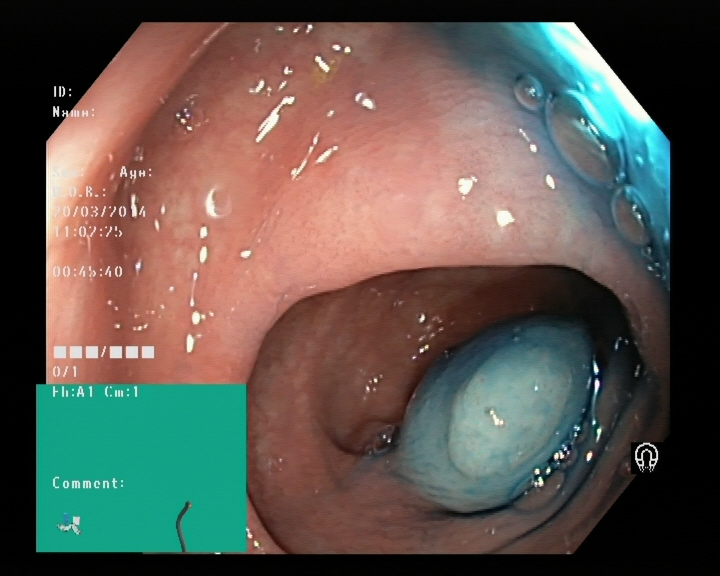
\includegraphics[width=4.5cm, height=4.5cm]{experiments/images/dyed-lifted-polyps.jpg}
       }
       \subfloat[\centering g]{
            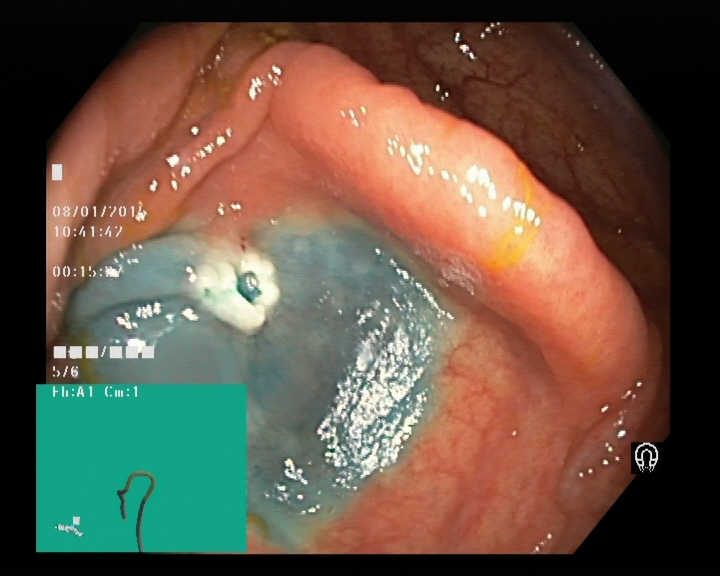
\includegraphics[width=4.5cm, height=4.5cm]{experiments/images/dyed-resection-margins.jpg}
        }
        \hspace{0mm}
       \subfloat[\centering g]{
            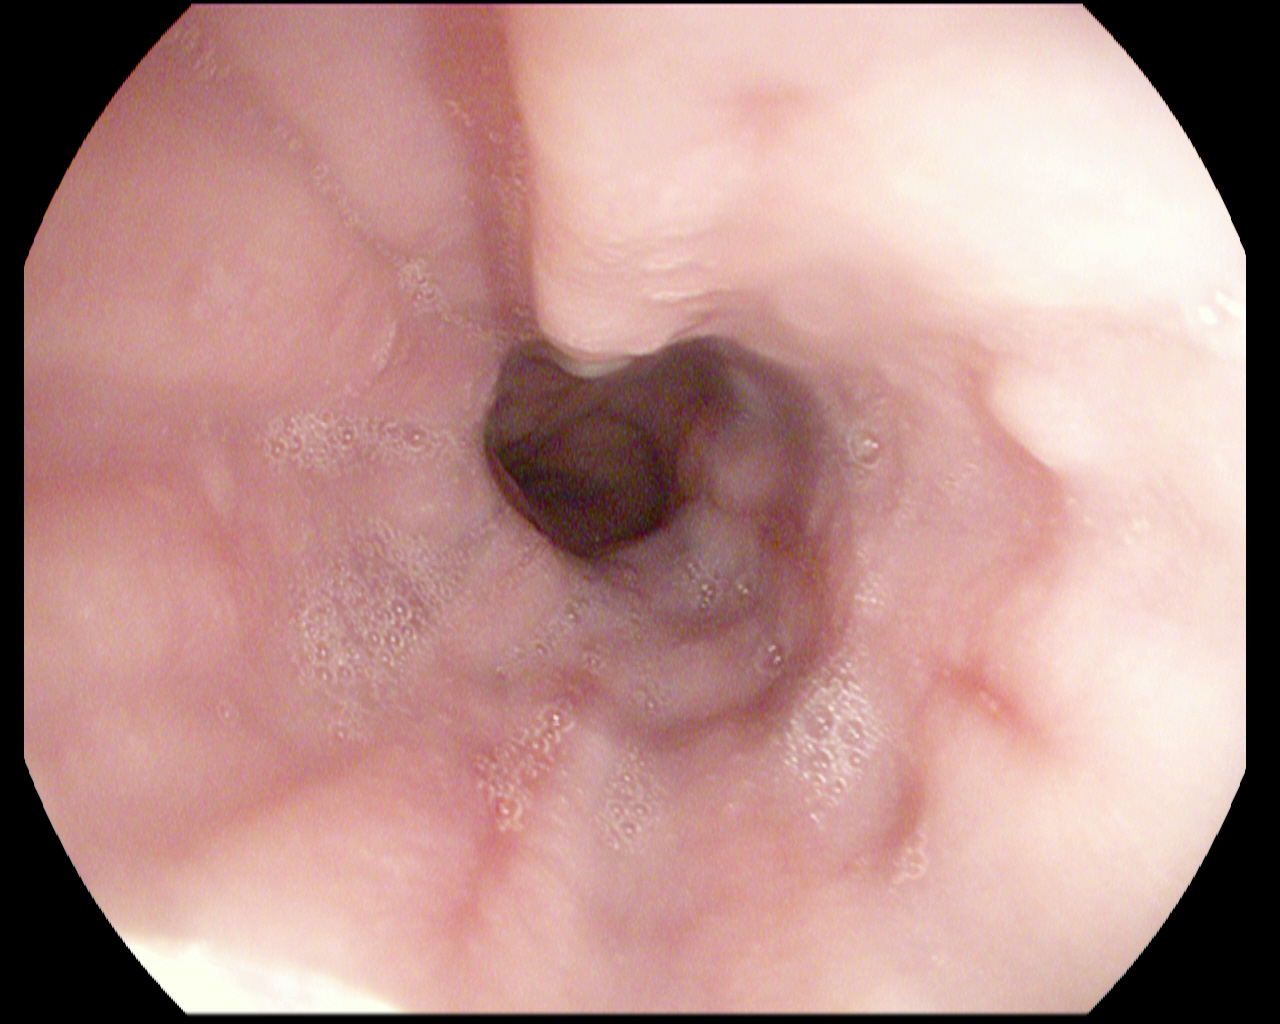
\includegraphics[width=4.5cm, height=4.5cm]{experiments/images/esophagitis.jpg}
        }
        \subfloat[\centering g]{
            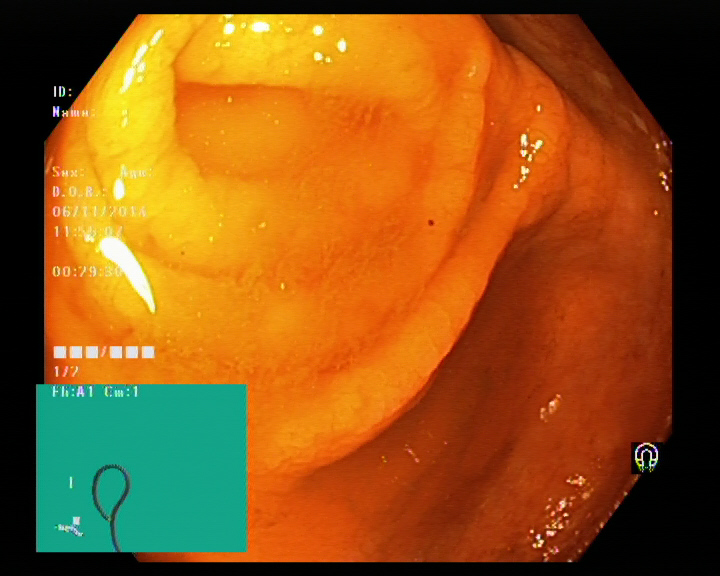
\includegraphics[width=4.5cm, height=4.5cm]{experiments/images/normal-cecum.jpg}
        }
        \hspace{0mm}
       \subfloat[\centering g]{
            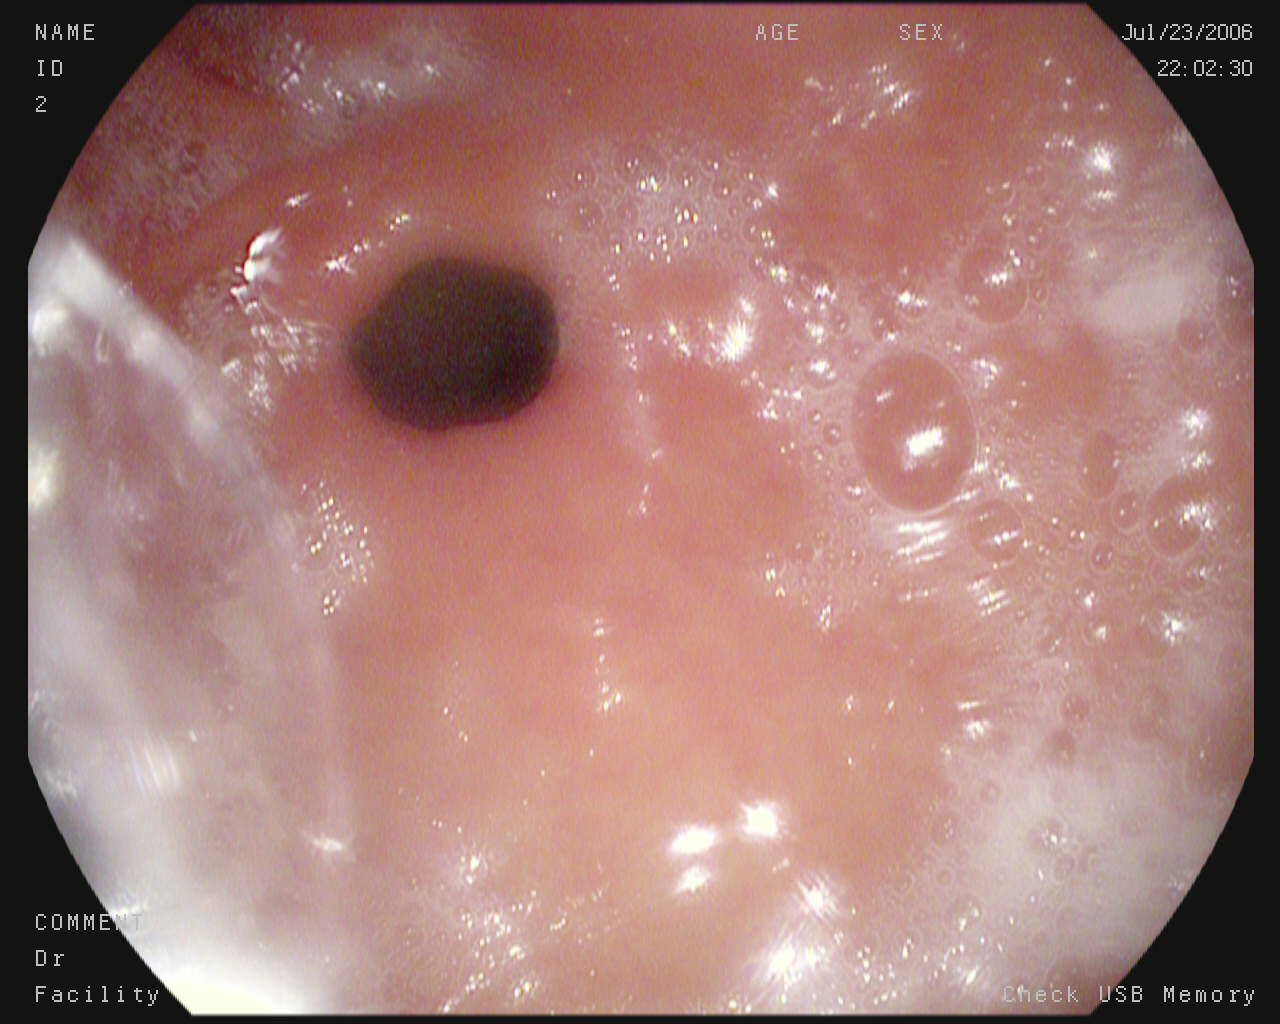
\includegraphics[width=4.5cm, height=4.5cm]{experiments/images/normal-pylorus.jpg}
       }
        \subfloat[][\centering g]{
            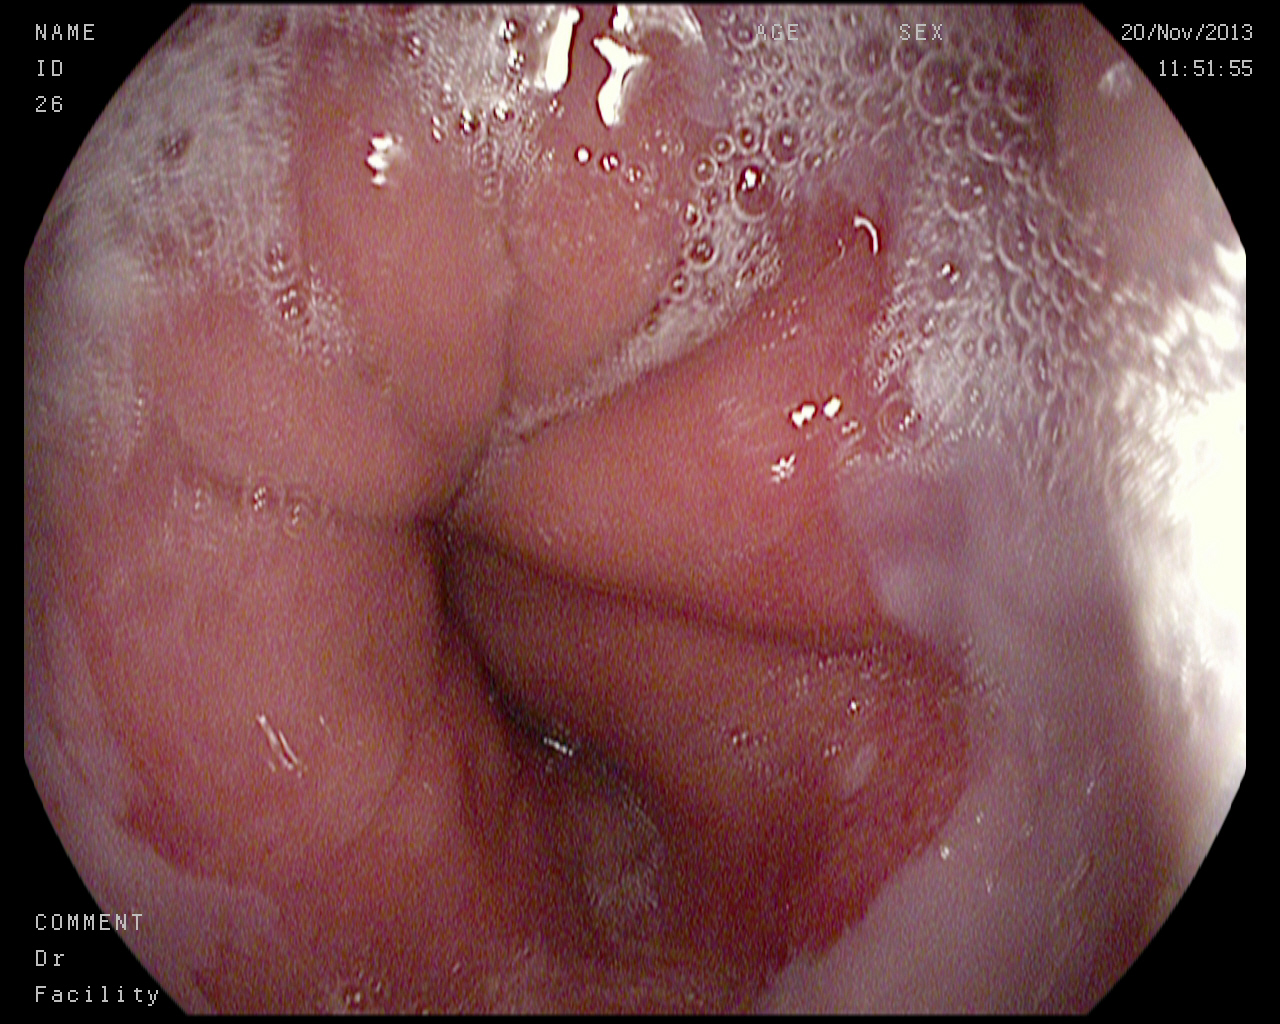
\includegraphics[width=4.5cm, height=4.5cm]{experiments/images/normal-z-line.jpg}
        }
        \hspace{0mm}
        \subfloat[\centering g]{
           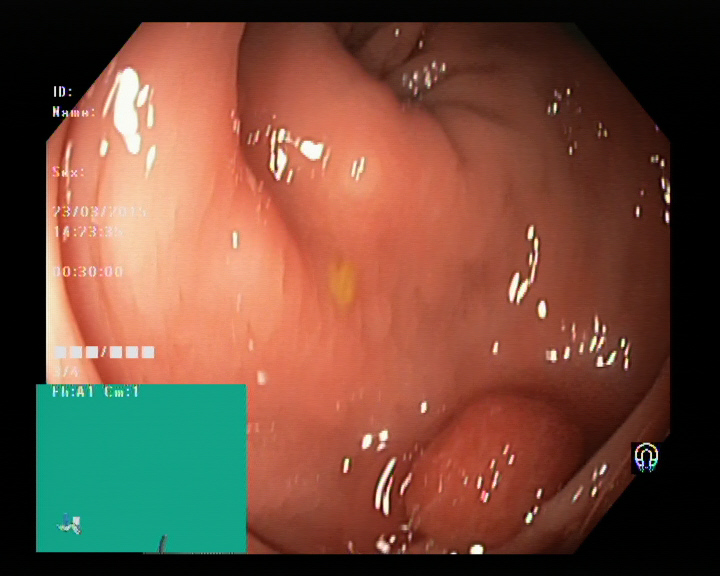
\includegraphics[width=4.5cm, height=4.5cm]{experiments/images/polyps.jpg}
        }
       \subfloat[\centering g]{
            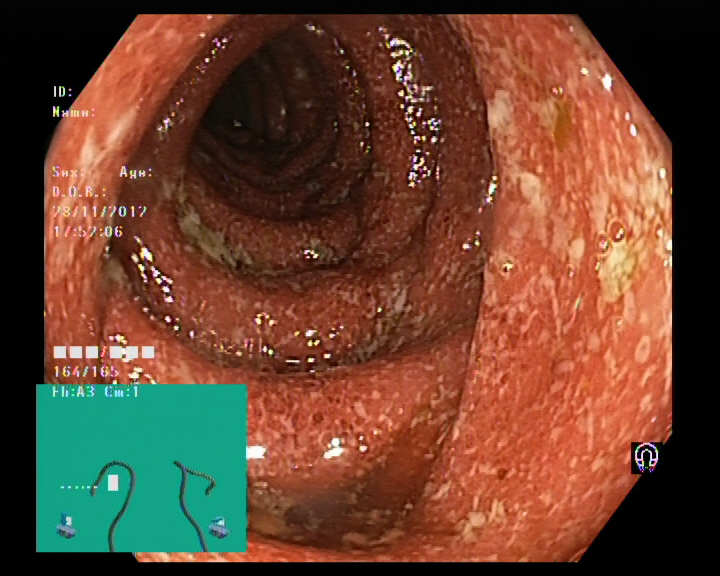
\includegraphics[width=4.5cm, height=4.5cm]{experiments/images/ulcerative-colitis.jpg}
        }
       \caption{Same image from the z-line with four different inpainting attempts. Each image is re-sized to fit in the figure.}
        \label{fig:images_16}
    \end{figure}
\fi
    %=============================================


To discern the results of our experiments we introduce multiple metrics and tables to get an indication of our success. 
The main dataset we used for training, Kvasir, was split into k number of folds, using k-fold cross-validation. 
K-fold cross-validation is a tool used in statistics and machine learning to help to get an accurate representation of the data based on an average of the dataset.  In machine learning, it is a powerful tool that can help with adapting to new datasets and prevent overfitting. 
Take the Kvasir dataset containing 8000 images with 1000 images from each class. We can choose a value for the number of folds, 'k', to be 6. This means that we split our dataset into six pieces before training.  With the six pieces, we assign one of them as a test set, and we assign the four other for training and validation. We then train our data five times, using four folds for training and the last fold for validation during training. For each training run we rotate the validation set, so each of the five folds is used for validation once. \todo{img of k fold}

The advantage of this method is that we maximise the utility of the dataset. We find the distribution of the dataset that hopefully covers the most significant range of the unseen data. 

\subsection{presantation of data, confusion matrix}
With k-fold cross-validation, we end up with the dataset that scored the highest during the final validation step.  There are multiple ways to calculate metrics for how well a dataset is doing,  but they all are a comparison of the predicted class versus the true class.  
Take for instance the case with the 8-class dataset Kvasir, where we predict an image to be of class 3, which in the real world be normal-z-line, while the actual True class is 5, and this might be esophagitis.\todo{rewrite}

We can represent this as 
\begin{verbatim}
[3, 5] 
\end{verbatim}.
Storing value pairs like this can very quickly get cluttered and unorganised.
The most common way to store these value pairs is to use a confusion matrix.  We initiate the matrix as a \textit{NxN} matrix where N is the total number of classes.
\begin{verbatim}
 [  0  0   0   0   0   0   0   0]
 [  0  0   0   0   0   0   0   0]
 [  0  0   0   0   0   0   0   0]
 [  0  0   0   0   0   0   0   0]
 [  0  0   0   0   0   0   0   0]
 [  0  0   0   0   0   0   0   0]
 [  0  0   0   0   0   0   0   0]
 [  0  0   0   0   0   0   0   0]
\end{verbatim} 
After we have initisialised the confusion matrix, we add each value pair as to the matrix at is corresoponding postition.  Given the pair \begin{verbatim} [3, 5]  \end{verbatim} we add one to the posistion corresoponding to (x=3,y=5).  Another example could be given the pair where we guessed class 0 and the true class was 0 (\begin{verbatim}[0, 0] \end{verbatim}), we add one to the matrix at position (x=0,y=0). Witch 2 examples we get the following confusion matrix.
\begin{verbatim}
 [  1  0   0   0   0   0   0   0]
 [  0  0   0   0   0   0   0   0]
 [  0  0   0   0   0   0   0   0]
 [  0  0   0   0   0   0   0   0]
 [  0  0   0   0   0   0   0   0]
 [  0  0   0   1   0   0   0   0]
 [  0  0   0   0   0   0   0   0]
 [  0  0   0   0   0   0   0   0]
\end{verbatim}
As we fill in the matrix with more predictions we can start to draw conclusions from it. After appoximently 1600 evaluations, our result might at the end look like this.
\begin{verbatim}
 [195  50   0   0   0   0   2   1]
 [  4 148   1   0   0   0   0   0]
 [  0   0 152   0   3  40   0   5]
 [  0   1   0 198   0   0  13   4]
 [  0   0   0   0 195   1   5   2]
 [  0   0  47   0   1 159   0   0]
 [  1   0   0   0   0   0 172   8]
 [  0   1   0   2   1   0   8 180]
\end{verbatim}
We can see that the highest numbers lies around the diagonal. This means that most of our results were classified correctly as values at the diagonal is the same x and y values, and subsequently a correct prediction. 
We can also discern something about the four primary metrics associated with a value in the matrix.\\

\textbf{True Positive (TP): } True positive for a specific class is when it is predicted positive, and the True label is also positive.  In the Kvasir dataset, we have a True positive result if, for the class polyp, we predict a polyp.\\

\textbf{True Negative (TN): } True Negative is the opposite of true positive. Given the class Polyp from the Kvasir dataset, we guess that the image is not a polyp when the True label is non-polyp. 

\textbf{False Positive (FP): } False positive is, given a True label we predict False. We often call this type of error a "Type 1 error".   In the polyp case, this is the case where we predict a polyp given no polyp present.


\textbf{False Negative (FN): } False positive is the case where we fail to predict the class when it is True. This type of error is often called "Type 2 error". False Negative is, in our case, the least desirable outcome for our classes with pathological findings like Esophagitis, Polyps and Ulcerative Colitis.

For our multiclass confusion table, we can look at the four metrics like this
\todo{https://i.stack.imgur.com/AuTKP.png}

%\begin{table}[]
%\begin{tabular}{llll}
%                            & \multicolumn{3}{l}{Predicted label} \\
%\multirow{3}{*}{True label} &            & True      & False      \\
%                            & True       & 5         & 7          \\
%                            & False      & 2         & 10        
%\end{tabular}
%\end{table}  

\subsection{common Metrics}
When evaluating our results, we use a set of common metrics used in the field of statistics and machine learning.  The metrics are Recall (REC), Precision (PREC), Specificity (SPEC), Accuracy (ACC), Matthews correlation coefficient (MCC), and F1 score (F1). 


\vspace{5px}
\textbf{Accuracy:}  Accuracy is one of the simplest metrics to understand. It describes how many of our predictions were correct out of the total predictions made. It is the most common metric given its simplicity both in calculation and understanding. 
In general when our data is balanced, and we only have a few classes, we can get away with using accuracy. 
In this project, we use accuracy during the training step as a metric of success.
 \begin{equation}
ACC=\frac{TP+TN}{TP+TN+FP+FN}
\end{equation}

\vspace{5px}
\textbf{Recall:}  Recall is the probability of detection \todo{ "Detector Performance Analysis Using ROC Curves – MATLAB & Simulink Example". www.mathworks.com. Retrieved 11 August 2016.}. In a binary classification set, it measures the proportion of actual positives that are correctly identified as such. 
For our medical image classification, this metric can help us understand how our algorithms work by looking at classes where we have small anomalies in the images, like the case with polyps.
\begin{equation}
TPR=\frac{TP}{TP+FN}
\end{equation}

\vspace{5px}
\textbf{Specificity:} Specificity measures the proportions of our samples that were correctly identified as negative, when the true class were also negative. 
\begin{equation}
TPR=\frac{TN}{TN+FP}
\end{equation}

\vspace{5px}
\textbf{Precision:}



\vspace{5px}
\textbf{F1 score:}

\vspace{5px}
\textbf{Matthews correlation coefficient:}

\subsection{Singleclass vs Multiclass Metrics}

The metrics presented are, in general, a solid way to present the validity of a model. However, not all metrics presented is the same when switching between single and multiclass classification.  Metrics like Accuracy is designed to work for multiclass classification, given that there is only one way to calculate the score.
\begin{equation}
\frac{sum(diag(covariance_matrix))}{sum(covariance_matrix))}
\end{equation}

The problem with multiclass metrics arises when there is more than one way to calculate the metrics needed, this can be for instance Recall and Specificity, where we have multiple ways to add together the classwise scores. The three most common ways to calculate the average are:

\textbf{Micro average}: calculates the mean value of each of the binary metrics and averages the result over the total number of samples. 
Micro average ignores all class frequencies and gives us a metric based on all samples gathered. Micro-averaging may be preferred in multilabel settings, including multiclass classification where a majority class is to be ignored.\\

\textbf{Macro average}: calculates the mean of each of the binary metrics, giving the same weight to each of the classes. Macro average gives importance to classes with few samples, and infrequent classes play the same roles as frequent ones. The disadvantage with Macro average is the fact that in the real world some classes often plays a more significant role than others, and doing especially bad on one of the classes can worsen the total result. \\

\textbf{Weighted average} calculates the mean of each of the binary metrics but gives a weighted sum for each of the scores before it is averaged. 
The weight of each class depends on the size of the true data samples.
The weighted average gives us the advantage that small classes still count more than it would with for instance Micro average, but since it depends on the number of samples from each class it can end up more or less as a black box during calculation.
Weighted average gives us the best of both worlds, but it lacks the intuitiveness from the two other classes. \\

With the three methods presented, we have chosen to Macro average our results. While both Macro and Weighted average would give a good indication given that not all our datasets are balanced, we argue that the weighted average would give metrics that are harder to explain when we are working on datasets with unbalanced classes.

In addition to looking at the Macro average of precision and recall, we want to look at specific cases of the classification.  In many cases, we have multiple classes, where we are most interested in just one or a handful of the classes shown. 
For instance, a focus we have in this thesis is to give a score on how predictable polyp detection is, and on that case, we want to discuss the True positive rate (TPR) of the polyp detection and not the TPR of the non-polyp classes. 

Take for instance the matrix shown in \todo{fig}\\
\begin{verbatim}
[[10 1]
 [3 12]]
\end{verbatim}
Here we can calculate the weighted average recall to be \textbf{x}. This can be an interesting observation in itself, but often the first or second True label is much more important relative to the other.  In a more practical example: We are more interested in finding areas with polyps when we know they are present, compared knowing there is not a polyp in an area when none are present. 

These Metrics becomes a more prominent topic when it comes to inpainting. With inpainting, we take areas with no relevant information and makes it into areas that are similar to the rest of the image. Given that we can inpaint over polyps by mistake, or that we might train our classifiers to not look in certain areas when classifying, we have an interest if also comparing single cases of recall and precision included to the average values.







\section{Setup of experiments}
We propose the following hypothesis.
\vspace{10px}

\begin{verbatim}
When classifying images, we will get the best result when we have images with the least amount of sparse information. 
Hence by removing areas with sparse information, we will see an increase in classification performance compared to not removing areas.
\end{verbatim}

and

\begin{verbatim}
When training a classifier, we will get a higher mode of generalisation of our results when removing dataset specific artefacts 
compared to not removing artefacts.
\end{verbatim}


In this thesis, we will set up our experiments to test our two hypothesises. 

\section{format of experiments}
    \subsection{Inpaint}
    \subsection{Classifying}
    
\section{Inpainting Kvasir}
    \subsection{Black corners}
    \subsection{Green square}
    \subsection{Text}
    \subsection{Combination}
    \subsection{Random masking}
    
\section{Kvasir -  CVC612}
\section{Kvasir -  CVC 12k}
\section{Kvasir -  CVC356}

\section{Summary
}
